\documentclass[12pt]{article}
\usepackage[margin=2.5cm]{geometry}
\usepackage{enumerate}
\usepackage{amsfonts}
\usepackage{amsmath}
\usepackage{fancyhdr}
\usepackage{amsmath}
\usepackage{amssymb}
\usepackage{amsthm}
\usepackage{mdframed}
\usepackage{graphicx}
\usepackage{subcaption}
\usepackage{adjustbox}
\usepackage{listings}
\usepackage{xcolor}
\usepackage{booktabs}
\usepackage[utf]{kotex}
\usepackage{hyperref}
\usepackage{accents}

\definecolor{codegreen}{rgb}{0,0.6,0}
\definecolor{codegray}{rgb}{0.5,0.5,0.5}
\definecolor{codepurple}{rgb}{0.58,0,0.82}
\definecolor{backcolour}{rgb}{0.95,0.95,0.92}

\lstdefinestyle{mystyle}{
    backgroundcolor=\color{backcolour},
    commentstyle=\color{codegreen},
    keywordstyle=\color{magenta},
    numberstyle=\tiny\color{codegray},
    stringstyle=\color{codepurple},
    basicstyle=\ttfamily\footnotesize,
    breakatwhitespace=false,
    breaklines=true,
    captionpos=b,
    keepspaces=true,
    numbers=left,
    numbersep=5pt,
    showspaces=false,
    showstringspaces=false,
    showtabs=false,
    tabsize=1
}

\lstset{style=mystyle}

\pagestyle{fancy}
\renewcommand{\headrulewidth}{0.4pt}
\lhead{CSC 343}
\rhead{Worksheet 13 Solution}

\begin{document}
\title{CSC343 Worksheet 13 Solution}
\maketitle

\begin{enumerate}[1.]
    \item

    \begin{enumerate}[a)]

        \item

        \begin{tabular}{|c|c|c|c|c|}
            \hline
            A & B & C & D & E\\
            \hline
            $a$ & $b$ & $c$ & $d_1$ & $e_1$\\
            \hline
            $a_1$ & $b$ & $c$ & $d$ & $e_2$\\
            \hline
            $a$ & $b_1$ & $c$ & $d_2$ & $e$\\
            \hline
        \end{tabular}

        \bigskip

        \underline{\textbf{Step 1 ($B \to E$):}}

        \bigskip

        \begin{tabular}{|c|c|c|c|c|}
            \hline
            A & B & C & D & E\\
            \hline
            $a$ & $b$ & $c$ & $d_1$ & $e_1$\\
            \hline
            $a_1$ & $b$ & $c$ & $d$ & $e_1$\\
            \hline
            $a$ & $b_1$ & $c$ & $d_2$ & $e$\\
            \hline
        \end{tabular}

        \bigskip

        \underline{\textbf{Step 2 ($CE \to A$):}}

        \bigskip

        \begin{tabular}{|c|c|c|c|c|}
            \hline
            A & B & C & D & E\\
            \hline
            $a$ & $b$ & $c$ & $d_1$ & $e_1$\\
            \hline
            $\color{red}a$ & $b$ & $c$ & $d$ & $e_1$\\
            \hline
            $a$ & $b_1$ & $c$ & $d_2$ & $e$\\
            \hline
        \end{tabular}

        \bigskip

        So in this case, an example of an instance of $R$ that is not lossless
        is:

        \bigskip

        \begin{tabular}{|c|c|c|c|c|}
            \hline
            Title & Studio Name & President & Year & President Address\\
            \hline
            Toy Story & Pixar & Steve Jobs & 2000 & 123 ABC Street\\
            \hline
            Star Wars & Fox & Lachlan Murdoch & 1977 & Hollywood\\
            \hline
            Return of the Jedi & Fox & Lachlan Murdoch & 1983 & Hollywood\\
            \hline
        \end{tabular}

        \bigskip

        \begin{itemize}
            \item $S_1 = \{A,B,C\}$

            \bigskip

            \begin{tabular}{|c|c|c|c|c|}
                \hline
                Title & Studio Name & President\\
                \hline
                Toy Story & Pixar & Steve Jobs\\
                \hline
                Star Wars & Fox & Lachlan Murdoch\\
                \hline
                Return of the Jedi & Fox & Lachlan Murdoch\\
                \hline
            \end{tabular}

            \item $S_2 = \{C,D,E\}$

            \bigskip

            \begin{tabular}{|c|c|c|c|c|}
                \hline
                President & Year & President Address\\
                \hline
                Steve Jobs & 2000 & 123 ABC Street\\
                \hline
                Lachlan Murdoch & 1977 & Hollywood\\
                \hline
                Lachlan Murdoch & 1983 & Hollywood\\
                \hline
            \end{tabular}

            \item $S_3 = \{C,E,A\}$

            \bigskip

            \begin{tabular}{|c|c|c|c|c|}
                \hline
                Title & President & President Address\\
                \hline
                Toy Story & Steve Jobs & 123 ABC Street\\
                \hline
                Star Wars & Lachlan Murdoch & Hollywood\\
                \hline
                Return of the Jedi & Lachlan Murdoch & Hollywood\\
                \hline
            \end{tabular}

            \item $S_1 \bowtie S_2$

            \begin{tabular}{|c|c|c|c|c|}
                \hline
                Title & Studio Name & President & Year & President Address\\
                \hline
                Toy Story & Pixar & Steve Jobs & 2000 & 123 ABC Street\\
                \hline
                Star Wars & Fox & Lachlan Murdoch & 1977 & Hollywood\\
                \hline
                Star Wars & Fox & Lachlan Murdoch & 1983 & Hollywood\\
                \hline
                Return of the Jedi & Fox & Lachlan Murdoch & 1977 & Hollywood\\
                \hline
                Return of the Jedi & Fox & Lachlan Murdoch & 1983 & Hollywood\\
                \hline
            \end{tabular}

            \item $S_1 \bowtie S_2 \bowtie S_3$

            \begin{tabular}{|c|c|c|c|c|}
                \hline
                Title & Studio Name & President & Year & President Address\\
                \hline
                Toy Story & Pixar & Steve Jobs & 2000 & 123 ABC Street\\
                \hline
                Star Wars & Fox & Lachlan Murdoch & 1977 & Hollywood\\
                \hline
                Star Wars & Fox & Lachlan Murdoch & 1983 & Hollywood\\
                \hline
                Return of the Jedi & Fox & Lachlan Murdoch & 1977 & Hollywood\\
                \hline
                Return of the Jedi & Fox & Lachlan Murdoch & 1983 & Hollywood\\
                \hline
            \end{tabular}

        \end{itemize}

        \bigskip

        \underline{\textbf{Notes:}}

        \bigskip

        \begin{itemize}
            \item Decomposition: The good bad and ugly

            \begin{enumerate}[1)]
                \item \textbf{Elimination of Anomalies} by decomposition as in Section 3
                \item \textbf{Recoverability of Information} Can we recover the original relation
                from the tuples in its decomposition?
                \item \textbf{Preservation of Dependences (lossless join):} Can we be sure that after reconstructing the original relation
                from the decompositions, the original FD's satisfy?
            \end{enumerate}

            \bigskip

            \textbf{BCNF:} $\to$ satisfies 1) and 2) \color{red}Not good. NONO\color{black}


            \item The Chase Test for Lossless Join
            \begin{itemize}
                \item Tests whether the decomposition is lossless
            \end{itemize}

            \bigskip

            \textbf{Input:}

            \begin{itemize}
                \item A relation $R$
                \item A decomposition of $R$
                \item A set of functional dependencies
            \end{itemize}

            \bigskip

            \textbf{Output:}

            \begin{itemize}
                \item Whether the decomposition is loseless or not
                \item $\Pi_{S_1}(R) \bowtie \Pi_{S_2}(R) \bowtie \cdots \Pi_{S_i}(R) = R$
            \end{itemize}

            \bigskip

            \underline{\textbf{Three things to remember:}}

            \begin{enumerate}[1.]
                \item The natural join is associate and commutative
                \item Any tuple $t$ in $R$ is surely in $\pi_{S_1}(R) \bowtie \pi_{S_2}(R) \bowtie \cdots \bowtie \pi_{S_k}(R)$.
                \item We have to check to see any tuple in the $\pi_{S_1}(R) \bowtie \pi_{S_2}(R) \bowtie \cdots \bowtie \pi_{S_k}(R)$.
            \end{enumerate}

            \bigskip

            \underline{\textbf{Example:}}

            \bigskip

            $S_1 = \{A,D\}$, $S_2 = \{B,C\}$, $S_3 = \{A,C\}$

            \bigskip

            $A \to B$, $B \to C$, $CD \to A$

            \begin{center}
            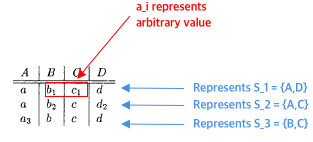
\includegraphics[width=0.7\linewidth]{images/worksheet_13_solution_1.png}
            \end{center}

            \bigskip

            \underline{\textbf{Step 1: $A \to B$}}

            \bigskip

            Set the value $b$ with the same value of $a$ to be the same. (e.g. $b_2 \to b_1$)

            \bigskip

            \begin{center}
            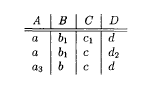
\includegraphics[width=0.7\linewidth]{images/worksheet_13_solution_2.png}
            \end{center}


            \bigskip

            \underline{\textbf{Step 2: $B \to C$}}

            \bigskip

            Set the value $c$ with the same value of $b$ to be the same. (e.g. $b_2 \to b_1$)

            \bigskip

            \begin{center}
            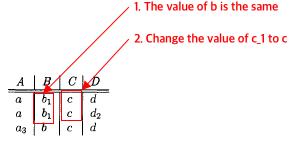
\includegraphics[width=0.7\linewidth]{images/worksheet_13_solution_3.png}
            \end{center}

            \bigskip

            \underline{\textbf{Step 3: $CD \to A$}}

            \bigskip

            Set the value $a$ with the same value of $c$ and $d$ to be the same. (e.g. $a_3 \to a$)

            \bigskip

            \begin{center}
            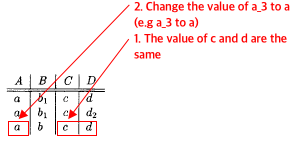
\includegraphics[width=0.7\linewidth]{images/worksheet_13_solution_4.png}
            \end{center}

            \bigskip

            So, we can conclude the join is lossless.

        \end{itemize}

        \item

        \begin{tabular}{|c|c|c|c|c|}
            \hline
            A & B & C & D & E\\
            \hline
            $a$ & $b$ & $c$ & $d_1$ & $e_1$\\
            \hline
            $a_1$ & $b$ & $c$ & $d$ & $e_2$\\
            \hline
            $a$ & $b_1$ & $c$ & $d_2$ & $e$\\
            \hline
        \end{tabular}

        \bigskip

        \underline{\textbf{Step 1 ($AC \to E$):}}

        \bigskip

        \begin{tabular}{|c|c|c|c|c|}
            \hline
            A & B & C & D & E\\
            \hline
            $a$ & $b$ & $c$ & $d_1$ & $\color{red}e$\\
            \hline
            $a_1$ & $b$ & $c$ & $d$ & $e_2$\\
            \hline
            $a$ & $b_1$ & $c$ & $d_2$ & $e$\\
            \hline
        \end{tabular}

        \bigskip

        \underline{\textbf{Step 2 ($BC \to D$):}}

        \bigskip

        \begin{tabular}{|c|c|c|c|c|}
            \hline
            A & B & C & D & E\\
            \hline
            $a$ & $b$ & $c$ & $\color{red}d$ & $\color{red}e$\\
            \hline
            $a_1$ & $b$ & $c$ & $d$ & $e_2$\\
            \hline
            $a$ & $b_1$ & $c$ & $d_2$ & $e$\\
            \hline
        \end{tabular}

        \bigskip

        $a,b,c,d,e$ exists. So by the Chast test, the decomposition of $R(A,B,C,D,E): AC \to E, BC \to D$
        into $\{A,B,C\}$, $\{B,C,D\}$, $\{A,C,E\}$ is lossless.

        \item

        \begin{tabular}{|c|c|c|c|c|}
            \hline
            A & B & C & D & E\\
            \hline
            $a$ & $b$ & $c$ & $d_1$ & $e_1$\\
            \hline
            $a_1$ & $b$ & $c$ & $d$ & $e_2$\\
            \hline
            $a$ & $b_1$ & $c$ & $d_2$ & $e$\\
            \hline
        \end{tabular}

        \underline{\textbf{Step 1 ($A \to D$):}}

        \bigskip

        \begin{tabular}{|c|c|c|c|c|}
            \hline
            A & B & C & D & E\\
            \hline
            $a$ & $b$ & $c$ & $d_1$ & $e_1$\\
            \hline
            $a_1$ & $b$ & $c$ & $d$ & $e_2$\\
            \hline
            $a$ & $b_1$ & $c$ & $\color{red}d_1$ & $e$\\
            \hline
        \end{tabular}

        \underline{\textbf{Step 2 ($D \to E$):}}

        \bigskip

        \begin{tabular}{|c|c|c|c|c|}
            \hline
            A & B & C & D & E\\
            \hline
            $a$ & $b$ & $c$ & $d_1$ & $\color{red}e$\\
            \hline
            $a_1$ & $b$ & $c$ & $d$ & $e_2$\\
            \hline
            $a$ & $b_1$ & $c$ & $\color{red}d_1$ & $e$\\
            \hline
        \end{tabular}

        \bigskip

        \underline{\textbf{Step 3 ($B \to D$):}}

        \bigskip

        \begin{tabular}{|c|c|c|c|c|}
            \hline
            A & B & C & D & E\\
            \hline
            $a$ & $b$ & $c$ & $\color{red}d$ & $\color{red}e$\\
            \hline
            $a_1$ & $b$ & $c$ & $d$ & $e_2$\\
            \hline
            $a$ & $b_1$ & $c$ & $\color{red}d$ & $e$\\
            \hline
        \end{tabular}

        \bigskip

        $a,b,c,d,e$ exists. So by the Chast test, the decomposition of $R(A,B,C,D,E): A \to D, D \to E, B \to D$
        into $\{A,B,C\}$, $\{B,C,D\}$, $\{A,C,E\}$ is lossless.

        \item

        \begin{tabular}{|c|c|c|c|c|}
            \hline
            A & B & C & D & E\\
            \hline
            $a$ & $b$ & $c$ & $d_1$ & $e_1$\\
            \hline
            $a_1$ & $b$ & $c$ & $d$ & $e_2$\\
            \hline
            $a$ & $b_1$ & $c$ & $d_2$ & $e$\\
            \hline
        \end{tabular}

        \underline{\textbf{Step 1 ($A \to D$):}}

        \bigskip

        \begin{tabular}{|c|c|c|c|c|}
            \hline
            A & B & C & D & E\\
            \hline
            $a$ & $b$ & $c$ & $d_1$ & $e_1$\\
            \hline
            $a_1$ & $b$ & $c$ & $d$ & $e_2$\\
            \hline
            $a$ & $b_1$ & $c$ & $\color{red}d_1$ & $e$\\
            \hline
        \end{tabular}

        \bigskip

        \underline{\textbf{Step 2 ($CD \to E$):}}

        \bigskip

        \begin{tabular}{|c|c|c|c|c|}
            \hline
            A & B & C & D & E\\
            \hline
            $a$ & $b$ & $c$ & $d_1$ & $\color{red}e$\\
            \hline
            $a_1$ & $b$ & $c$ & $d$ & $e_2$\\
            \hline
            $a$ & $b_1$ & $c$ & $\color{red}d_1$ & $e$\\
            \hline
        \end{tabular}

        \bigskip

        \underline{\textbf{Step 3 ($E \to D$):}}

        \bigskip

        \begin{tabular}{|c|c|c|c|c|}
            \hline
            A & B & C & D & E\\
            \hline
            $a$ & $b$ & $c$ & $d_1$ & $\color{red}e$\\
            \hline
            $a_1$ & $b$ & $c$ & $d$ & $e_2$\\
            \hline
            $a$ & $b_1$ & $c$ & $\color{red}d_1$ & $e$\\
            \hline
        \end{tabular}

        \bigskip

        So in this case, the relation is not lossless.

        \bigskip

        An example of an instance of $R$ that is not lossless
        is:

        \bigskip

        \begin{tabular}{|c|c|c|c|c|}
            \hline
            Phone ID & Grade & Student Name & Phone \# & Physical Address\\
            \hline
            1 & 89 & John Doe & 111-222-3333 & 123 ABC Street\\
            \hline
            2 & 89 & John Doe & 222-222-3333 & 123 ABC Street\\
            \hline
            1 & 62 & Josh Doe & 111-222-3333 & 123 ABC Street\\
            \hline
            3 & 94 & Frank McKay & 444-555-6666 & 234 ABC Street\\
            \hline
        \end{tabular}

        \bigskip

        \begin{itemize}
            \item $S_1 = \{A,B,C\}$

            \bigskip

            \begin{tabular}{|c|c|c|}
                \hline
                Phone ID & Grade & Student Name\\
                \hline
                1 & 89 & John Doe\\
                \hline
                2 & 89 & John Doe\\
                \hline
                1 & 62 & Josh Doe\\
                \hline
                3 & 94 & Frank McKay\\
                \hline
            \end{tabular}

            \item $S_2 = \{C,D,E\}$

            \bigskip

            \begin{tabular}{|c|c|c|c|c|}
                \hline
                Student Name & Phone \# & Physical Address\\
                \hline
                John Doe & 111-222-3333 & 123 ABC Street\\
                \hline
                John Doe & 222-222-3333 & 123 ABC Street\\
                \hline
                Josh Doe & 111-222-3333 & 123 ABC Street\\
                \hline
                Frank McKay & 444-555-6666 & 234 ABC Street\\
                \hline
            \end{tabular}

            \item $S_3 = \{A,C,E\}$

            \bigskip

            \begin{tabular}{|c|c|c|c|c|}
                \hline
                Phone ID & Student Name & Physical Address\\
                \hline
                1 & John Doe & 123 ABC Street\\
                \hline
                2 & John Doe & 123 ABC Street\\
                \hline
                1 & Josh Doe & 123 ABC Street\\
                \hline
                3 & Frank McKay & 234 ABC Street\\
                \hline
            \end{tabular}

            \item $S_1 \bowtie S_2$

            \begin{tabular}{|c|c|c|c|c|}
                \hline
                Phone ID & Grade & Student Name & Phone \# & Physical Address\\
                \hline
                1 & 89 & John Doe & 111-222-3333 & 123 ABC Street\\
                \hline
                2 & 89 & John Doe & 111-222-3333 & 123 ABC Street\\
                \hline
                1 & 89 & John Doe & 222-222-3333 & 123 ABC Street\\
                \hline
                2 & 89 & John Doe & 222-222-3333 & 123 ABC Street\\
                \hline
                1 & 62 & Josh Doe & 111-222-3333 & 123 ABC Street\\
                \hline
                3 & 94 & Frank McKay & 444-555-6666 & 234 ABC Street\\
                \hline
            \end{tabular}

            \item $S_1 \bowtie S_2 \bowtie S_3$

            \begin{tabular}{|c|c|c|c|c|}
                \hline
                Phone ID & Grade & Student Name & Phone \# & Physical Address\\
                \hline
                1 & 89 & John Doe & 111-222-3333 & 123 ABC Street\\
                \hline
                2 & 89 & John Doe & 111-222-3333 & 123 ABC Street\\
                \hline
                1 & 89 & John Doe & 222-222-3333 & 123 ABC Street\\
                \hline
                2 & 89 & John Doe & 222-222-3333 & 123 ABC Street\\
                \hline
                1 & 62 & Josh Doe & 111-222-3333 & 123 ABC Street\\
                \hline
                3 & 94 & Frank McKay & 444-555-6666 & 234 ABC Street\\
                \hline
            \end{tabular}

        \end{itemize}


    \end{enumerate}

    \item

    The sets of FDs in 1.b) and 1.c) are the ones where the dependencies are
    preserved from decomposition.

    \item

    \begin{enumerate}[a)]
        \item

        \begin{enumerate}[i)]
            \item Find 3NF Violations

            \bigskip
            \color{red}
            \begin{itemize}
                \item $\{A,B\}^+ = \{A,B\}$
                \begin{itemize}
                    \item Violates 3NF
                    \item Doesn't have $C$ required for $AB \to C$
                    \item Second and third don't imply first
                \end{itemize}
                \item $\{C\}^+ = \{C\}$
                \begin{itemize}
                    \item Violates 3NF
                    \item Doesn't have $D$ required for $C \to D$
                    \item First and third don't imply second
                \end{itemize}
                \item $\{D\}^+ = \{D\}$
                \begin{itemize}
                    \item Violates 3NF
                    \item Doesn't have $A$ required for $D \to A$
                    \item First and second don't imply third
                \end{itemize}
            \end{itemize}

            \color{black}

            \item Decompose relations, as necessary, into collections as a part of 3NF

            \bigskip

            \begin{enumerate}[1.]
                \item Find a minimal basis for $F$, say $G$

                \bigskip

                \color{red}
                A possible FD to simplify is $AB \to C$. But since $\{B\}^+ = \{B\}$,
                and $\{A\}^+ = \{A\}$, and both has $C$ missing, the FD cannot be
                simplified further.

                \bigskip

                so the minimal basis for $F$ is

                \bigskip

                $AB \to C$, $C \to D$, $D \to A$
                \color{black}

                \bigskip

                \item For each functional dependency $X \to A$ in $G$, use $XA$
                as the schema of one of the relations in the decomposition

                \bigskip

                \color{red}
                $S_1(A,B,C)$, $S_2(C,D)$, $S_3(D,A)$
                \color{black}

                \bigskip

                \item If none of the relation schemas from Step 2 is a superkey for $R$,
                add another relation whose schema is a key for $R$. And drop redundant relations.

                \bigskip

                \color{red}
                The keys for this relation are $\{A,B,C\}, \{B,C,D\}, \{D,A,B\}$

                \bigskip

                The attributes in $S_1(A,B,C)$ is a key. So, this step can be skipped.
                \color{black}

            \end{enumerate}
        \end{enumerate}

        \bigskip

        \underline{\textbf{Notes:}}

        \bigskip

        \begin{itemize}
            \item 3NF
            \begin{itemize}
                \item Definition
                \begin{itemize}
                    \item A elation $R$ is in 3NF if

                    \bigskip

                    For each nontrivial FD, the left side is a superkey (BCNF), or
                    the right side consists of prime attributes only.
                \end{itemize}
                \item Our expectation after decomposing are:
                \begin{enumerate}[1.]
                    \item Elimination of Anomalies
                    \item Recoverability of Information (Recovering original relation after decomposition)
                    \item Preservation of Information (Recovering original tuples after decomposition)
                \end{enumerate}

                \bigskip

                Key: \color{red}3NF guarentees 2) and 3) but not 1)\color{black}
            \end{itemize}
            \item Violations
            \begin{itemize}
                \item $X \to A$ violates 3NF if and only if $X$ is not a superkey
                and also $A$ is not prime.

                \bigskip

                \textbf{Prime Attributes} are attributes that are part of a key.

                \bigskip
            \end{itemize}
            \item Synthesis algorithm for 3NF Schemas
            \begin{enumerate}[1.]
                \item Check if the FD's are minimal
                \begin{itemize}
                    \item To verify, we should show that we cannot eliminate any of FD's.
                    That is, using algorithm 3.7, no two of the FD's imply the third
                \end{itemize}
                \item Find a minimal basis for $F$, say $G$
                \item For each functional dependency $X \to A$ in $G$, use $XA$
                as the schema of one of the relations in the decomposition
                \item If none of the relation schemas from Step 3 is a superky for $R$,
                add another relation whose schema is a key for $R$. And drop redundant relations.
            \end{enumerate}

            \bigskip

            \underline{\textbf{Example:}}

            \bigskip

            $R(A,B,C,D,E): AB \to C, C \to B, A \to D$

            \bigskip

            \begin{enumerate}[1.]
                \item Check if the FD's are minimal
                \begin{itemize}
                    \item To verify, we should show that we cannot eliminate any of FD's.
                    That is, using algorithm 3.7, no two of the FD's imply the third
                \end{itemize}

                \bigskip

                \color{red}
                \begin{enumerate}[1)]
                    \item $\{A,B\}^+$

                    \bigskip

                    Using the FDs $C \to B$, $A \to D$, we have $\{A,B\}^+ = \{A,B,D\}$.

                    \bigskip

                    Since $C$ is required for $AB \to C$, we can conclude second
                    and third doesn't imply the first

                    \item $\{C\}^+$

                    \bigskip

                    Using the FDs $AB \to C$, $A \to D$, we have $\{C\}^+ = \{C\}$.

                    \bigskip

                    Since $B$ is required for $C \to B$ but not in $\{C\}^+ = \{C\}$, we can conclude first
                    and third doesn't imply the second

                    \item $\{A\}^+$

                    \bigskip

                    Using the FDs $AB \to C$, $C \to D$, we have $\{A\}^+ = \{A\}$.

                    \bigskip

                    Since $D$ is required for $C \to D$ but not in $\{A\}^+ = \{A\}$, we can conclude first
                    and second doesn't imply the third

                \end{enumerate}

                \color{black}


                \item Find a minimal basis for $F$, say $G$

                \bigskip

                \color{red}
                $AB \to C$, $C \to B$ and $A \to D$
                \color{black}

                \item For each functional dependency $X \to A$ in $G$, use $XA$
                as the schema of one of the relations in the decomposition

                \bigskip

                \color{red}
                $S_1(A,B,C)$, $S_2(C,B)$, $S_3(A,D)$
                \color{black}

                \bigskip

                \item If none of the relation schemas from Step 3 is a superky for $R$,
                add another relation whose schema is a key for $R$. And drop redundant relations.

                \bigskip

                \color{red}

                Take all combinations of attributes $A,B,C,D,E$. We have $\{A,B,C\}$ and
                $\{A,B,E\}$ as keys.

                \bigskip

                Thus, adding one, the extra relation we have is $S_4(A,B,E)$.

                \bigskip

                And since $B,C$ in $S_2(B,C)$ is also in $S_1(A,B,C)$, $S_2$ needs to be dropped.

                \bigskip

                So, we have $S_1(A,B,C)$, $S_3(A,D)$, $S_4(A,B,E)$

                \color{black}
            \end{enumerate}

        \end{itemize}

        \item

        \begin{enumerate}[i)]
            \item Find 3NF Violations

            \bigskip

            \color{red}
            \begin{itemize}
                \item $\{B\}^+ = \{B,C,D\}$
                \begin{itemize}
                    \item Violates 3NF
                    \item Doesn't have $C$ required for $B \to C$
                    \item Doesn't have $C$ required for $B \to D$
                    \item Second and third don't imply first
                \end{itemize}
            \end{itemize}
            \color{black}

            \item Decompose relations, as necessary, into collections as a part of 3NF

            \bigskip

            \begin{enumerate}[1.]
                \item Find a minimal basis for $F$, say $G$

                \bigskip

                \color{red}
                $B \to D$ and $B \to C$
                \color{black}

                \bigskip

                \item For each functional dependency $X \to A$ in $G$, use $XA$
                as the schema of one of the relations in the decomposition

                \bigskip

                \color{red}
                $S_1(B,D)$, $S_2(B,C)$
                \color{black}

                \bigskip

                \item If none of the relation schemas from Step 2 is a superkey for $R$,
                add another relation whose schema is a key for $R$. And drop redundant relations.

                \bigskip

                \color{red}
                The keys for this relation are $\{A,B\}$

                \bigskip

                So, the new sets of relation are $S_1(B,D)$, $S_2(B,C)$, $S_3(A,B)$
                \color{black}

                \bigskip

            \end{enumerate}
        \end{enumerate}

        \item

        \begin{enumerate}[i)]
            \item Find 3NF Violations

            \bigskip

            \color{red}
            \begin{itemize}
                \item $\{A,B\}^+ = \{A,B\}$
                \begin{itemize}
                    \item Violates 3NF
                    \item Doesn't have $C$ required for $AB \to C$
                    \item Second, third and fourth don't imply first
                \end{itemize}

                \item $\{B,C\}^+ = \{B,C\}$
                \begin{itemize}
                    \item Violates 3NF
                    \item Doesn't have $D$ required for $BC \to D$
                    \item first, third and fourth don't imply second
                \end{itemize}

                \item $\{C,D\}^+ = \{C,D\}$
                \begin{itemize}
                    \item Violates 3NF
                    \item Doesn't have $A$ required for $CD \to A$
                    \item first, second and fourth don't imply third
                \end{itemize}

                \item $\{A,D\}^+ = \{A,D\}$
                \begin{itemize}
                    \item Violates 3NF
                    \item Doesn't have $B$ required for $AD \to B$
                    \item first, second and third don't imply fourth
                \end{itemize}
            \end{itemize}
            \color{black}

            \item Decompose relations, as necessary, into collections as a part of 3NF

            \bigskip

            \begin{enumerate}[1.]
                \item Find a minimal basis for $F$, say $G$

                \bigskip

                \color{red}
                $AB \to C$, $BC \to D$, $CD \to A$ and $AD \to B$
                \color{black}

                \bigskip

                \item For each functional dependency $X \to A$ in $G$, use $XA$
                as the schema of one of the relations in the decomposition

                \bigskip

                \color{red}
                $S_1(A,B,C)$, $S_2(B,C,D)$, $S_3(C,D,A)$, $S_4(A,D,B)$
                \color{black}

                \bigskip

                \item If none of the relation schemas from Step 2 is a superkey for $R$,
                add another relation whose schema is a key for $R$. And drop redundant relations.

                \bigskip

                \color{red}
                The keys for this relation are $\{A,B,C\}$, $\{B,C,D\}$, $\{C,D,A\}$,$\{A,D,B\}$

                \bigskip

                The attributes in $S_1(A,B,C)$ is a key. So, this step can be skipped.
                \color{black}

                \bigskip

            \end{enumerate}
        \end{enumerate}

        \item

        \begin{enumerate}[i)]
            \item Find 3NF Violations

            \bigskip

            \color{red}
            No 3NF violations exist
            \color{black}

        \end{enumerate}


        \item

        \begin{enumerate}[i)]
            \item Find 3NF Violations

            \bigskip

            \color{red}
            \begin{itemize}
                \item $\{A,B\}^+ = \{A,B,D\}$
                \begin{itemize}
                    \item Violates 3NF
                    \item Doesn't have $C$ required for $AB \to C$
                    \item Second and third don't imply first
                \end{itemize}

                \item $\{D,E\}^+ = \{D,E,C\}$
                \begin{itemize}
                    \item Violates 3NF
                    \item Doesn't have $D$ required for $DE \to C$
                    \item first and third don't imply second
                \end{itemize}

                \item $\{B\}^+ = \{B\}$
                \begin{itemize}
                    \item Violates 3NF
                    \item Doesn't have $D$ required for $B \to D$
                    \item first and second don't imply third
                \end{itemize}
            \end{itemize}
            \color{black}

            \item Decompose relations, as necessary, into collections as a part of 3NF

            \bigskip

            \begin{enumerate}[1.]
                \item Find a minimal basis for $F$, say $G$

                \bigskip

                \color{red}
                $AB \to C$, $DE \to C$ and $B \to D$
                \color{black}

                \bigskip

                \item For each functional dependency $X \to A$ in $G$, use $XA$
                as the schema of one of the relations in the decomposition

                \bigskip

                \color{red}
                $S_1(A,B,C)$, $S_2(D,E,C)$, $S_3(B,D)$
                \color{black}

                \bigskip

                \item If none of the relation schemas from Step 2 is a superkey for $R$,
                add another relation whose schema is a key for $R$. And drop redundant relations.

                \bigskip

                \color{red}
                The keys for this relation is $\{A,B,E\}$

                \bigskip

                So, the new sets of relation are $S_1(A,B,C)$, $S_2(D,E,C)$, $S_3(B,D)$, $S_4(A,B,E)$
                \color{black}

                \bigskip

            \end{enumerate}
        \end{enumerate}


    \end{enumerate}

\end{enumerate}

\end{document}